\documentclass[10pt,a4paper]{article}
\usepackage{amsmath,amssymb,amsthm,graphicx}
\usepackage{bm,enumitem,textcomp,algorithm,xspace,mathtools,subfig,thmtools,thm-restate}
\usepackage[noend]{algpseudocode}
\usepackage[classfont=bold]{complexity}
\usepackage[svgnames]{xcolor}
\usepackage{hyperref}
\usepackage[capitalise,noabbrev,nameinlink]{cleveref}
\graphicspath{{items/}}
\theoremstyle{plain}
\newtheorem{theorem}{Theorem}[section]
\newtheorem{lemma}[theorem]{Lemma}
\newtheorem{corollary}[theorem]{Corollary}
\newtheorem{proposition}[theorem]{Proposition}
\newtheorem{claim}[theorem]{Claim}

\theoremstyle{remark}
\newtheorem{remark}[theorem]{Remark}
\newtheorem{example}[theorem]{Example}

\theoremstyle{definition}
\newtheorem{definition}[theorem]{Definition}
\newcommand{\pa}[1]{}
\newcommand{\kr}[1]{}
%%%
%%% Generic math macros
%%%

% equation with def above
\newcommand\defeq{\stackrel{\mathclap{\normalfont\mbox{\scriptsize{def}}}}{=}}

\DeclareMathOperator*{\supp}{supp}
\DeclareMathOperator*{\conn}{conn}
\DeclareMathOperator{\Char}{char}
\newcommand{\eps}{\varepsilon}

\newcommand{\eqcomma}{\enspace ,}
\newcommand{\eqperiod}{\enspace .}
\newcommand{\disjointunion}{\overset{.}{\cup}}
\newcommand{\expec}[2][]{\mathbb{E}_{#1}[#2]}
\newcommand{\prob}[2][]{\Pr_{#1}[#2]}
\newcommand{\Prob}[2][]{\Pr_{#1} \bigl[ #2 \bigr]}
\providecommand{\abs}[1]{\lvert#1\rvert}
\providecommand{\Abs}[1]{\bigl\lvert#1\bigr\rvert}
\providecommand{\ABS}[1]{\left\lvert#1\right\rvert}
\newcommand{\set}[1]{\{#1\}}
\newcommand{\setdescr}[2]{\{\,#1 \mid #2\,\}}
\newcommand{\floor}[1]{\lfloor #1 \rfloor}
\newcommand{\ceil}[1]{\lceil #1 \rceil}
\newcommand\restrict[2]{{% we make the whole thing an ordinary symbol
  \left.\kern-\nulldelimiterspace % automatically resize the bar with \right
  #1 % the function
  \vphantom{\big|} % pretend it's a little taller at normal size
  \right|_{#2} % this is the delimiter
  }}
% indicator
\usepackage{bbm}
\newcommand{\ind}[1]{\mathbbm{1}{\set{#1}}}

% cal of everything
\newcommand{\calA}{\mathcal{A}}
\newcommand{\calB}{\mathcal{B}}
\newcommand{\calC}{\mathcal{C}}
\newcommand{\calD}{\mathcal{D}}
\newcommand{\calE}{\mathcal{E}}
\newcommand{\calF}{\mathcal{F}}
\newcommand{\calG}{\mathcal{G}}
\newcommand{\calH}{\mathcal{H}}
\newcommand{\calI}{\mathcal{I}}
\newcommand{\calJ}{\mathcal{J}}
\newcommand{\calK}{\mathcal{K}}
\newcommand{\calL}{\mathcal{L}}
\newcommand{\calM}{\mathcal{M}}
\newcommand{\calN}{\mathcal{N}}
\newcommand{\calO}{\mathcal{O}}
\newcommand{\calP}{\mathcal{P}}
\newcommand{\calQ}{\mathcal{Q}}
\newcommand{\calR}{\mathcal{R}}
\newcommand{\calS}{\mathcal{S}}
\newcommand{\calT}{\mathcal{T}}
\newcommand{\calU}{\mathcal{U}}
\newcommand{\calV}{\mathcal{V}}
\newcommand{\calW}{\mathcal{W}}
\newcommand{\calX}{\mathcal{X}}
\newcommand{\calY}{\mathcal{Y}}
\newcommand{\calZ}{\mathcal{Z}}


% R, N, Z, F etc
\renewcommand{\C}{\mathbb{C}}
\renewcommand{\E}{\mathbb{E}}
\newcommand{\PE}{\mathbb{\widetilde{E}}}
\renewcommand{\R}{\mathbb{R}}
\newcommand{\N}{\mathbb{N}}
\newcommand{\Z}{\mathbb{Z}}
\newcommand{\F}{\mathbb{F}}

\newcommand{\trace}{\mathsf{tr}}
\newcommand{\Var}{\mathsf{Var}}


\DeclareMathOperator{\Deg}{\sf{Deg}}
\DeclareMathOperator{\Size}{\sf{Size}}
\newcommand{\RefuteDeg}[2]{\Deg(#2 \vdash_{\text{\tiny #1}} \, \perp)}
\newcommand{\RefuteSize}[2]{\Size(#2 \vdash_{\text{\tiny #1}} \, \perp)}

% pseudo-distribution
\newcommand{\pedef}{\tilde{\mathbb{E}}}
\newcommand{\pe}[2][]{\pedef_{#1}[#2]}

% monotone anything
\newcommand{\mon}{{\mathsf{mon}}}

% circuit size
\DeclareMathOperator{\csize}{\calC}
\DeclareMathOperator{\cmonsize}{\csize_{\mathsf{mon}}}

% Misc
\DeclareMathOperator{\hw}{\texttt{hw}}

% out and in for the g fns
\newcommand{\gout}{g^\mathrm{out}}
\newcommand{\ginone}{g^\mathrm{in_1}}
\newcommand{\gintwo}{g^\mathrm{in_2}}

% Notation related to the expander graphs
\DeclareMathOperator{\idx}{\texttt{ind}}
\DeclareMathOperator{\neigh}{\textbf{Neigh}}
  

% subformula
\newcommand{\subformula}{$ is a variable substitution of $}

% the selectors
\DeclareMathOperator{\sel}{\mathsf{Sel}}

% the circuit formula
\newcommand{\vars}[1]{\mathsf{#1}}
\DeclareMathOperator{\circuit}{Circuit}
\DeclareMathOperator{\outwire}{\vars{Out}}
\DeclareMathOperator{\inwire}{\vars{In}}
\DeclareMathOperator{\isneg}{\vars{IsNeg}}
\DeclareMathOperator{\isand}{\vars{IsAnd}}
\DeclareMathOperator{\isor}{\vars{IsOr}}
\DeclareMathOperator{\isfromconst}{\vars{IsFromConst}}
\DeclareMathOperator{\isfromvar}{\vars{IsFromInput}}
\DeclareMathOperator{\isfromgate}{\vars{IsFromGate}}
\DeclareMathOperator{\constval}{\vars{ConstantValue}}
\DeclareMathOperator{\isvar}{\vars{IsInput}}
\DeclareMathOperator{\isgate}{\vars{IsGate}}

% axioms for cref
\crefname{axiom}{Axiom}{Axioms}
\Crefname{axiom}{Axiom}{Axioms}

\crefname{axioms}{Axioms}{Axioms}
\Crefname{axioms}{Axioms}{Axioms}
% old notation -- might need if we create an appendix:
% cnf <-> poly encoding
\DeclareMathOperator{\isvarless}{\vars{IsInput^{\le}}}
\DeclareMathOperator{\isgateless}{\vars{IsGate^{\le}}}
\title{Sum-of-Squares degree and size lower bounds for general MCSP}
\author{Per Austrin, Kilian Risse}
\date{doi:10.4230/LIPIcs.CCC.2023.31; CC BY4.0}
\begin{document}
\maketitle
\setcounter{section}{1}
\noindent\textit{Editorial note.} Original authors: Per Austrin and Kilian Risse. arXiv:2311.12994v1 (2023-11-21), https://arxiv.org/abs/2311.12994v1. Creative Commons Attribution4.0, https://creativecommons.org/licenses/by/4.0/.\par\medskip
\noindent\textit{Editorial note.} Selected complete native author main theorem/proof/context, original circuit diagrams and bibliography in standalone layout. Input files explicitly flattened into source spans, unused frontmatter/font packages omitted. No mathematical changes or new proofs. Original CC BY4.0 license retained.\par\medskip
\noindent\textit{Allowed standard prerequisites (editorial).}\begin{itemize}
\item Explicit unbalanced expanders, expander XOR SoS degree lower bound and SoS size-degree tradeoff. Exact cited author statements in preliminaries retained; all local substitution/restriction support supplied in full.
\end{itemize}\medskip
\section{Preliminaries}
\label{sec:preliminaries}

All logarithms are in base $2$.  For integers $n \ge 1$ we write
$[n] = \set{1, 2, \ldots, n}$ and for a set $U$ we denote the power
set of $U$ by $2^{U}$. Further, for a set $V \subseteq U$ we let
$\overline V$ be the complement of $V$ with respect to $U$, that is,
$\overline V = U \setminus V$. We write
$\binom{[n]}{\ell} \subseteq \set{0,1}^n$ for the set of binary
strings with Hamming weight $\ell$. For a string
$\alpha \in \set{0,1}^n$ we let
$|\alpha| = \sum_{i \in [n]} \alpha_i$.

We sometimes want to supress dependencies on constants and write
$f(n, \eps) \in O_\eps\big(g(n, \eps)\big)$, respectively
$f(n, \eps) \in \Omega_\eps\big(g(n, \eps)\big)$, to mean that there
exists a function $c(\eps) > 0$ such that there is an $n_0$ and for all
$n \ge n_0$ it holds that $f(n, \eps) \le c(\eps) \cdot g(n, \eps)$,
respectively $f(n, \eps) \ge c(\eps)\cdot g(n, \eps)$.

\begin{definition}\label{def:explicit}
  A sequence of bipartite graphs $\set{G_n=(U_n, V_n, E_n)}_{n\in \N}$
  with $\deg(u) =d$ for all $u \in U_n$ is \emph{explicit} if there is
  an algorithm that given $(n, u, j)$, where $n \in \N, u \in U_n$ and
  $j\in [d]$, computes the $j$th neighbor of vertex $u$ in the graph
  $G_n$ in time $\poly(\log n + \log |U| + \log d)$.
\end{definition}

From now on it is understood that whenever we talk about an explicit
graph we actually mean to say that there is a sequence of explicit
graphs with above properties.

For a graph $G = (V, E)$ and $W \subseteq V$ we denote by
\[
  N(W) = \setdescr{u \in V \setminus W}{(w,u) \in E \text{ for some } w
    \in W}
\]
the set of neighbors of $W$.

\begin{definition}
  A bipartite graph $G = (U, V, E)$ is an $(r, d, c)$-expander if every
  vertex $u \in U$ has degree $\deg(u) = d$ and every set
  $W \subseteq U$ of size $|W| \le r$ satisfies $|N(W)| \ge c \cdot |W|$.
\end{definition}

A key ingredient in our proofs is the following result on the
existence of strong explicit expanders.

\begin{theorem}[\cite{GUV09Unbalanced}]\label{thm:expander}
  For all constants $\gamma > 0$,
  every $M \in \N$, $r \le M$,
  and $\eps > 0$,
  there is an
  $N \le d^2 \cdot r^{1 + \gamma}$ and an
  explicit
  $(r, d, (1- \eps)d)$-expander
  $G=(U, V, E)$,
  with $|U| = M$,
  $|V| = N$, and
  $d = O\big( ((\log M)(\log r) / \eps )^{1+1/\gamma}\big)$.
\end{theorem}

\kr{Igor pointed this out:
  \url{https://eccc.weizmann.ac.il/report/2018/159/}. Quickly checking
  the parameters I believe it does not give anything better. Need to
  check more carefully}

For our purposes it is more relevant to compute the neighbor relation
$\neigh(u,v)$ indicating whether $(u, v) \in E$ rather than the
neighbor function as in \cref{def:explicit}, but this is an immediate
consequence of being able to compute the neighbor function.

\begin{claim}
  \label{claim:explicit neigh}
  If $G = (U, V, E)$ is explicit then the neighbor relation
  $\neigh: U \times V \rightarrow \{0,1\}$ is computable by a circuit
  of size
  $d \cdot \big( \poly(\log n + \log |U| + \log d) + 2 \log |V| + 1
  \big)$.
\end{claim}

% \pa{Added this fact, check that I was not too optimistic in claimed
  % size bound. Maybe add proof here.} \kr{checked.}

% Recall that this graph is explicit and hence there are
% circuits to compute the neighbor function
% $\Gamma: U \times [k] \rightarrow Z$.

% Each circuit $C_1, \ldots, C_z$ consists of $k$ circuits $\calD =
% \set{D_1, \ldots, D_k}$ that compute $\Gamma$ with the second input
% fixed to their corresponding index. On top of these circuits from
% $\calD$ we add a small circuit  $E_i$, which computes the following.
% Each circuit $D \in \calD$ outputs
% some index $j \in [z]$. The circuit $E_i$ outputs $1$ if and only if
% one of the $D \in \calD$ outputs the index $i$. The circuit $E_i$ is
% fairly small: for each circuit $D$ we require $2 \log z$ gates to
% check whether $D$ output $i$, and an additional $k$ gates to \emph{or}
% these outputs together. So in total each $E_i$ consists of
% $k (2\log z + 1)$ many gates.
% As the graph $G$ is explicit, we know that there is a circuit of size
% $\poly(n + \log k)$ computing $\Gamma$ and hence the size of all
% circuits in $\calD$ is bounded by $c_\alpha \cdot k \cdot n^c$, for
% some constant $c$, and $c_\alpha$ depending on $\alpha$. Hence we
% conclude that
% \begin{align}\label{eq:bound-a}
%  a = z \cdot \big(k (2\log z + 1) + c_\alpha \cdot k \cdot n^c\big) \eqperiod
% \end{align}


A slice function is a Boolean function $f$ such that there is a
$\ell \in [n]$ with $f(\alpha) = 0$ whenever $|\alpha| < \ell$, and
$f(\alpha) = 1$ whenever $|\alpha| > \ell$.  Note that all slice
functions are monotone.

The circuit complexity $\csize(f)$ of a Boolean function $f$ is the
size of the smallest circuit over the basis $\vee, \wedge$, and
$\lnot$ (with fan-in $2$). Similarly the monotone circuit
complexity $\cmonsize(f)$ of a monotone Boolean function $f$
is the size of the smallest circuit over the basis $\vee$, and
$\wedge$. We have the following useful inequality between these
measures.

\begin{lemma}[\cite{B82}]\label{lem:slice}
  If $g$ is any slice function on $n$ bits, then
  $\cmonsize(g) \le 2 \csize(g) + O(n^2 \log n)$.
\end{lemma}

Finally we also rely on the following simple claim.

\begin{claim}
  \label{claim:0 mod bool}
  Let $p: \R^n \rightarrow \R$ be a degree $d$ polynomial such that
  $p(x) = 0$ for all $x \in \{0,1\}^n$.  Then $p$ can be written as
  \[
    p(x) = \sum_{i \in [n]} q_i(x) \cdot (x_i^2-x_i)
  \]
  where each term in the sum has degree at most $d$.
\end{claim}

\begin{proof}[Proof sketch]
  We take the polynomial $p$ and multilinearize it, using the
  appropriate polynomial $x_i^2 - x_i$. Eventually we are left with a
  sum of polynomials of the form $q_i(x)\cdot(x_i^2 - x_i)$ and a
  multilinear polynomial $\tilde p(x)$ which is $0$ on all Boolean
  inputs.  As multilinear polynomials are a basis for Boolean
  functions this implies that $\tilde p(x)$ is equal to the $0$
  polynomial and hence the claim follows.
\end{proof}

\subsection{Sum of Squares}
\label{sec:known-SoS-results}

Let $\calP = \set{p_1 = 0, \ldots, p_m = 0}$ be a system of polynomial
equations over the set of variables
$X = \set{x_1, \ldots, x_n, \bar{x}_1, \ldots, \bar{x}_n}$.  Each
$p_i$ is called an \emph{axiom}, and throughout the paper we always
assume that $\calP$ includes all axioms $x_i^2 - x_i$ and
$\bar{x}_i^2 - \bar{x}_i$, ensuring that the variables are Boolean, as
well as the axioms $1 - x_i - \bar{x}_i$, making sure that the ``bar''
variables are in fact the negation of the ``non-bar'' variables.

%

\begin{definition}[Sum-of-Squares]
  \emph{Sum-of-Squares (SoS)} is a static, semi-algebraic proof
  system. An SoS proof of $f \ge 0$ from $\calP$ is a sequence of
  polynomials $\pi = (t_1, \ldots, t_m; s_1, \ldots, s_a)$ such that
  \begin{align*}
    \sum_{i \in [m]} t_i p_i +
    \sum_{i \in [a]} s^2_i = f \eqperiod %\label{eq:sos-def}
  \end{align*}
  The \emph{degree} of a proof $\pi$ is
  $\Deg(\pi) = \max \set{ \max_{i \in [m]} \deg(t_i) + \deg(p_i),
    \max_{i \in [a]} 2 \deg(s_i) }$, an \emph{SoS refutation of
    $\calP$} is an SoS proof of $-1 \ge 0$ from $\calP$, and the
  \emph{SoS degree to refute $\calP$} is the minimum degree of any SoS
  refutation of $\calP$: if we let $\pi$ range over all SoS
  refutations of $\calP$, we can write
  $\RefuteDeg{SoS}{\calP} = \min_\pi \Deg(\pi)$.  The \emph{size of an
    SoS refutation $\pi$}, $\Size(\pi)$, is the sum of the number of
  monomials in each polynomial in $\pi$ and the \emph{size of refuting
    $\calP$} is the minimum size over all refutations
  $\RefuteSize{SoS}{\calP} = \min_{\pi} \Size(\pi)$.
\end{definition}


Let us recall some well-known results about SoS. Given a bipartite
graph $G = (U, V, E)$, and $b \in \set{0,1}^{|U|}$ we denote by
$\Phi(G,b)$ the following XOR-CSP instance defined over $G$: for each
$v \in V$ there is a Boolean variable $x_v$, and for every vertex
$u \in U$ there is a constraint $\oplus_{v \in N(u)} x_v = b_u$.
We encode this in the obvious way as a system of polynomial equations: 
\begin{align*}
  \big\{
  \prod_{v \in N(u)} (1 - 2 \cdot x_v) = 1 - 2 \cdot b_u
  \mid u \in U
  \big\} \eqcomma
\end{align*}
along with the Boolean axioms and the negation axioms for the $x$
variables. The first theorem we need to recall is the classic lower
bounds for XOR-CSPs by Grigoriev.

\begin{theorem}[\cite{gri01xor}]\label{thm:sos-xor}
  For $n \in \N$, all $k = k(n)$ and $r = r(n)$ the following holds.
  Let $G = (U, V, E)$ be an $(r, k, 2)$-expander with $|V| = n$. Then
  for every $b \in \set{0,1}^{|U|}$ SoS requires degree $\Omega(r)$ to
  refute the claim that there is a satisfying assignment to
  $\Phi(G, b)$.
\end{theorem}

We also need to recall the size-degree tradeoff by Atserias and
Hakoniemi.

\begin{theorem}[\cite{AH18SosTradeoff}]\label{thm:tradeoff}
  Let $\calP$ be a system of polynomial equations over $n$ Boolean
  variables and degree at most $k$. If $d$ is the minimum degree
  SoS requires to refute $\calP$, then the minimum size of an SoS
  refutation of $\calP$ is at least $\exp(\Omega((d-k)^2/n))$.
\end{theorem}


\subsection{Restrictions}
\label{sec:restrictions}

Let $\calP = \set{p_1 = 0, \ldots, p_m = 0}$ be a system of polynomial
equations over the set of Boolean variables
$X = \set{x_1, \ldots, x_n, \bar{x}_1, \ldots, \bar{x}_n}$.
%
For a map
$\rho: \set{x_1, \ldots, x_n} \to \set{0,1, x_1, \ldots, x_n,
  \bar{x}_1, \ldots, \bar{x}_n}$ denote by $\restrict{\calP}{\rho}$
the system of polynomial equations $\calP$ restricted by $\rho$, i.e.,
\begin{align*}
\restrict{\calP}{\rho} = \set{ &p_1(\rho(x_1), \ldots, \rho(x_n)) = 0,\\
  &p_2(\rho(x_1), \ldots, \rho(x_n)) = 0,\\ &\vdots\\ &p_m(\rho(x_1),
  \ldots, \rho(x_n)) = 0 }\eqcomma
\end{align*}
where it is understood that $\rho(\bar x_i) = \overline{\rho(x_i)}$,
with the convention $\bar{\bar{x}}_i = x_i$, $\bar 0 = 1$ and vice
versa. Throughout the paper all our restrictions set the bar variables
to the negation of the non-bar variables. As such it makes sense to
treat the pair of variables $(x_i, \bar x_i)$ as one variable and we
say that $\calP$ has $n$ \emph{unset} variables.

\begin{definition}[Variable Substitution]
  We say that a system of polynomial equations $\calP'$ is a
  \emph{variable substitution of $\calP$} if there is a map
  $\rho: \set{x_1, \ldots, x_n} \to \set{0,1, x_1, \ldots, x_n,
    \bar{x}_1, \ldots, \bar{x}_n}$ such that
  $\calP' = \restrict{\calP}{\rho}$, where we ignore polynomial
  equations of the form $0=0$.
\end{definition}

The following well-known lemma states that a system of polynomial
equations $\calP$ is at least as hard as any of its variable substitutions.
\begin{lemma}\label{lem:subformula}
  Let $\calP, \calP'$ be systems of polynomial equations such that
  $\calP' \subformula \calP$. Then,
  \begin{enumerate}[label=$(\roman*)$]
  \item $\RefuteDeg{SoS}{\calP} \ge \RefuteDeg{SoS}{\calP'}$, and
  \item $\RefuteSize{SoS}{\calP} \ge \RefuteSize{SoS}{\calP'}$.
  \end{enumerate}
\end{lemma}
The lemma is easy to verify by considering an SoS refutation of
$\calP$ and hitting it with the appropriate variable substitution. The
restricted proof is now a refutation of $\calP'$ and it can be seen
that the degree/size of the restricted refutation is at most the
degree/size of the original refutation.

We also consider more general substitutions.

\begin{definition}[Polynomial Substitution]
  Functions
  $\rho: \set{x_1, \ldots, x_n} \rightarrow \R[x]_{\le k}$ that map
  variables to polynomials of degree at most $k$ are called
  \emph{polynomial substitutions}.
\end{definition}

For polynomial substitutions we have the following well-known lemma.

\begin{lemma}
  \label{lem:sos degree polynomial substitution}
  Let $\calP$ be a system of polynomial equations and let $\rho$ be a
  polynomial substitution mapping variables to polynomials of degree
  at most $k$. Then,
  $\RefuteDeg{SoS}{\calP} \ge
  \RefuteDeg{SoS}{\restrict{\calP}{\rho}}/k$.
\end{lemma}

This lemma can again be verified by considering a refutation of
$\calP$. Substitute each variable $x_i$ in the proof by
$\rho(x_i)$. This results in a refutation of $\restrict{\calP}{\rho}$,
whose degree is at most a factor $k$ larger than the degree of the
refutation of $\calP$.

\subsection{The Circuit Size Formula}
\label{sec:circuit-encoding}
The formula $\circuit_s(f)$ encodes the claim that the function $f$,
given as a truthtable $f \in \set{0, 1}^{2^n}$, can be computed by a
circuit of size $s$ over $n$ Boolean inputs $x_1, \ldots, x_n$. The
encoding is not essential but for concreteness let us fix one encoding
of this claim. We deviate from the encoding used by Razborov
\cite{Razborov98, Razborov04ResolutionLowerBoundsPM} and do not
present the formula as a propositional formula but rather as a system
of polynomial equations. In order to encode below constraints as a
constant width CNF formula, as done by Razborov, one needs to
introduce extension variables. Despite this difference it is not
difficult to see that our lower bound also works against the CNF
encoding. In \cref{sec:encoding} we directly show that a low degree
SoS refutation of the CNF encoding gives rise to a low degree SoS
refutation of the encoding used in this paper (see
\cref{prop:cnf-poly}). Thus a lower bound for our encoding implies a
lower bound for the CNF encoding. As the presentation is simpler in
the polynomial encoding, we present it as follows.

We also need to define the monotone version of $\circuit_s(f)$ denoted
by $\circuit^{\mathsf{mon}}_s(f)$. The later is a restriction of the
former with the $\isneg(v)$ (see below) variable, for all $v \in [s]$,
set to $0$. This forces the circuit to only contain $\land$ and $\lor$
gates, i.e., the circuit is monotone.

All variables introduced in the following are Boolean variables and we
implicitly add the Boolean axiom $y(1 - y) = 0$ for each variable $y$
and further implicitly introduce the ``bar variable'' $\bar{y}$ along
with the negation axiom $y = 1 - \bar{y}$ (and the corresponding
Boolean axiom) ensuring that $\bar{y}$ is always the negation of $y$.

Let us first describe the \emph{structure variables} which are used to
describe the circuit that supposedly computes the function $f$.

We view the $s$ gates as being indexed from $1$ to $s$ in topological
order with gate $s$ being the output.
For each gate $v \in [s]$ there are three variables $\isneg(v),
\isor(v), \isand(v)$ indicating the operation computed at
$v$. Similarly for a gate $v \in [s]$ and a wire $a \in \set{1,2}$ we
have variables $\isfromconst(v, a), \isfromvar(v, a), \isfromgate(v, a)$
indicating whether the input wire $a$ of $v$ is connected to a
constant, a variable or a gate.

Further, we have the variables $\constval(v, a)$, $\isvar(v, a, i)$
and $\isgate(v, a, u)$, for $a \in \set{1,2}$, $i \in [n]$ and
$u < v$, specifying the constant value, input $x_i$ or gate $u$, the
input wire $a$ of $v$ is connected to (assuming $a$ is connected to
the corresponding kind).

The second set of variables are the \emph{evaluation variables}, which
describe what value is computed at each $v$ on input
$\alpha = \alpha_1, \ldots, \alpha_n$ (i.e., we have $x_i = \alpha_i$).

For each gate $v \in [s]$ and assignment $\alpha \in \set{0,1}^n$ we
have a Boolean variable $\outwire_\alpha(v)$ indicating the value
computed at gate $v$ on input $\alpha$. The Boolean variable
$\inwire_{\alpha}(v, a)$ indicates the value brought to the vertex
$v \in [s]$ on wire $a \in \set{1,2}$ on input $\alpha$.

Note that there is a total of
$3s + 6s + 2s + 2sn + 2{s \choose 2} = \Theta(s^2+sn)$ structure
variables, and a total of $3 s 2^n$ evaluation variables, for a total
of $\Theta(s^2 + s 2^n)$ variables in $\circuit_s(f)$.

The formula consists of the following axioms. For the sake of
readability we omit some universal quantifiers: the variable
$a \in \set{1,2}$ in
\cref{eq:ax-from,eq:ax-in-gt,eq:ax-in-gt2,eq:prod-zero-in,eq:prod-zero-gate,eq:inwire-const,eq:inwire-var,eq:inwire-gate}
as well as the variable $\alpha \in \set{0,1}^n$ in
\cref{eq:inwire-const,eq:inwire-var,eq:inwire-gate,eq:ax-neg,eq:ax-or,eq:ax-and,eq:ax-correct}
are implicitly universally quantified.

Let us first describe
the axioms on the structure of the circuit. In the following
section we refer to this set of axioms as the \emph{structure
  axioms}. The first axioms ensure that every wire is connected to a
single kind
\begin{align}
  \label{eq:ax-from}
  \isfromconst(v, a) +
  \isfromvar(v, a) +
  \isfromgate(v, a) = 1 \quad
  \forall \, v \in [s] \eqcomma
\end{align}
and similarly the next axioms make sure that each gate is of
precisely one kind
\begin{align}
  \label{eq:ax-fn}
  \isneg(v) + \isor(v) + \isand(v) = 1
  \quad \forall \, v \in [s] \eqperiod
\end{align}
The final structure axioms ensure that the variables, which indicate
to what input or gate a fixed wire is connected to, always sum to one
(except for gate $1$ which cannot have any inputs from other gates)
\begin{align}
  \label{eq:ax-in-gt}
  \sum_{i = 1}^{n}\isvar(v,a,i) &= 1
  \quad \forall v \in [s], \text{ and}\\
  \label{eq:ax-in-gt2}
  \sum_{u = 1}^{v-1}\isgate(v,a,u) &= 1
  \quad \forall v \in [s] \setminus\{1\} \eqperiod
\end{align}
We further strengthen our encoding by adding the axioms
\begin{align}
  \label{eq:prod-zero-in}
  \isvar(v,a,i)\isvar(v,a,j) &= 0
  \quad\forall v \in [s],\, i < j \in [n], \text{ and}\\
  \label{eq:prod-zero-gate}
  \isgate(v,a,u)\isgate(v,a,u') &= 0
  \quad\forall u < u' < v \in [s] \eqperiod
\end{align}
Note that \cref{eq:prod-zero-in,eq:prod-zero-gate} are implied by
\cref{eq:ax-in-gt,eq:ax-in-gt2}. We add these axioms in order to argue
that a short refutation of the CNF encoding of this principle leads to
a short refutation of the present encoding.

The second group of axioms are the \emph{evaluation axioms} and they
ensure that the evaluation variables indeed compute the intended
values. We start by making sure that the wires carry the value
intended by the structure axioms. If a wire is connected to a
constant, then the evaluation variable associated with that wire
should always be equal to the constant
\begin{align}
  \label{eq:inwire-const}
  \isfromconst(v,a) \cdot
  \big( \inwire_{\alpha}(v,a) - \constval(v, a) \big) = 0 \eqcomma
\end{align}
and similarly in case if a wire is connected to an input or a gate
\begin{align}
  \label{eq:inwire-var}
  \isfromvar(v, a) \cdot \isvar(v, a, i) \cdot
  \big( \inwire_\alpha(v, a) - \alpha_i\big) &= 0
  \eqcomma\\
  \label{eq:inwire-gate}
  \isfromgate(v, a) \cdot \isgate(v, a, u) \cdot
  \big(\inwire_\alpha(v, a) - \outwire_\alpha(u)\big) &= 0 \eqperiod
\end{align}
The final set of evaluation axioms makes sure that the output
evaluation variable of a gate is correctly related to the input
evaluation variables:
\begin{align}
  \label{eq:ax-neg}
  \isneg(v) \cdot
  \outwire_{\alpha}(v)
  &=
    \isneg(v) \cdot
    \overline{\inwire_{\alpha}(v, 1)}\eqcomma\\
  \label{eq:ax-or}
  \isor(v) \cdot
  \outwire_{\alpha}(v)
  &=
    \isor(v)
    \cdot \big(
    1 -
    \overline{\inwire_{\alpha}(v, 1)} \cdot
    \overline{\inwire_{\alpha}(v, 2)}
    \big) \eqcomma\\
  \label{eq:ax-and}
  \isand(v) \cdot
  \outwire_{\alpha}(v)
  &=
    \isand(v) \cdot
    \inwire_{\alpha}(v, 1) \cdot
    \inwire_{\alpha}(v, 2) \eqperiod
\end{align}

Last but not least we have the axioms that ensure that the circuit
outputs the function specified by the truthtable
\begin{align}
  \label{eq:ax-correct}
  \outwire_{\alpha}(s) &= f(\alpha) \eqperiod
\end{align}

\section{On Circuits and Restrictions}
\label{sec:circ-rest}

Let $G=(U, V, E)$ be a bipartite graph with $U = \set{0,1}^n$ and
$V = [m]$. As in the XOR-CSP setup (\cref{sec:known-SoS-results}) we
think of vertices in $U$ as constraints and vertices in $V$ as
variables. More specifically, we think of each vertex $\alpha \in U$
as an \emph{xor} constraint over the variables in the neighborhood
$\oplus_{i \in N(\alpha)} v_i = b_\alpha$, for a constraint vector
$b \in \set{0,1}^U$. Given an assignment $\beta \in \set{0,1}^m$ to
the variables $V$, we let $f_{G, \beta}: U \rightarrow \set{0,1}$ be
the function defined by
$f_{G, \beta}(\alpha) = \oplus_{i \in N(\alpha)} v_i$.  In other
words, viewing $f_{G,\beta}$ as a vector in $\set{0,1}^U$, it is the
unique constraint vector such that the XOR-CSP instance, defined over
$G$, is satisfied by the assignment $\beta$. Let us denote the set of
all such constraint vectors that give rise to a satisfiable XOR-CSP
instance by
\[
  \calF_G = \set{f_{G, \beta} \,|\, \beta \in \set{0,1}^m} \eqperiod
\]
In order for SoS to refute an XOR-CSP instance defined over $G$,
it must prove that the given constraint vector is not in the set
$\calF_G$.

On the other hand in order for SoS to refute the formula $\circuit_s(f)$
it needs to show that there is no circuit of size at most $s$
computing $f$. That is, SoS needs to show that $f$ is not in the set
\[
  \calC_{\emptyset} =
  \set{
    T:
    \set{0,1}^n \rightarrow \set{0,1}
    \text{~such that~}
    \circuit_s(T)
    \text{~is satisfiable}
  } \eqperiod
\]
More generally, if we restrict $\circuit_s(f)$ by a restriction
$\rho$, then the proof system must prove that $f$ is not a member
of the family of truthtables
\[
  \calC_\rho =
  \set{
    T:
    \set{0,1}^n \rightarrow \set{0,1}
    \text{~such that~}
    \restrict{\circuit_s(T)}{\rho}
    \text{~is satisfiable}
  } \eqperiod
\]

In the following we show that there is a well-behaved restriction
$\rho$ such that $\calC_\rho = \calF_G$ for some explicit graphs
$G$. In other words, once we consider the restricted formula
$\restrict{\circuit_s(f)}{\rho}$, SoS needs to rule
out that $f$ is a valid right hand side of an XOR-CSP instance. But we
know that if $G$ is a moderate expander, then low degree SoS cannot
determine whether the XOR-CSP instance is satisfiable and hence we
obtain our lower bound.

Let us first formalize the properties we require from $\rho$. We start
off by restricting our attention to a certain natural class of variable
substitutions. Namely, we do not want that the structure of the circuit
depends on evaluation variables.

\begin{definition}[natural variable substitutions]
  A variable substitution $\rho$ to the variables of $\circuit_s(f)$ is
  \emph{natural} if there is \emph{no} structure variable $y$ such
  that $\rho(y)$ is an evaluation variable.
\end{definition}

In order to motivate the next definition, let us informally
describe the natural restriction $\rho$ and explain the properties of
$\rho$ we require.

For now we can think of $\rho$ as a restriction to the structure
variables (though for the size lower bounds we also need to restrict
some of the evaluation variables). Some set of $m$ structure variables remains
undetermined. Let us denote these variables by $y_1, \ldots, y_m$. We
intend to choose $\rho$ such that on a given input
$\alpha \in \set{0,1}^n$ to the circuit, it is forced to compute
$\oplus_{i \in N(\alpha)} y_i$.  In other words, given such a
restriction $\rho$, we are \emph{essentially} left with an XOR-CSP
problem over $G$, with right hand side $f$.  There is however a
difference in that the encoding is non-standard: the evaluation
variables act like extension variables that correspond to the
functions computed at each gate of the circuit. In order to argue that
the known degree lower bound for the XOR-CSP problem implies a degree
lower bound for the problem at hand, we need to get rid of these
extension variables. This can be done if the functions computed at the
gates are of low degree in the $y$ variables.

Recall from \cref{sec:restrictions} that a system of polynomial
equations $\calP$ has $n$ unset variables if there are $n$ tuples of
variables $(x, \bar x)$ such that at least one variable of each tuple
occurs in $\calP$ and all variables in these tuples are unset, i.e.,
they are not fixed to a constant.

\begin{definition}[$k$-determined]
  \label{def:determined}%
  Let $\rho$ be a variable substitution to the variables of
  $\circuit_s(f)$ and suppose that $\rho$ leaves $m$ structural
  variables $Y = \set{y_1, \ldots, y_m}$ unset.  Then $\rho$ is
  \emph{$k$-determined} if for every $v \in [s]$ and
  $\alpha \in \set{0,1}^n$ there are multilinear polynomials
  $$\gout_{v, \alpha}, \ginone_{v, \alpha}, \gintwo_{v, \alpha}:
  \set{0,1}^m \rightarrow \set{0,1}$$ depending on at most $k$
  variables such that the following holds. For all $T \in \calC_\rho$
  and all total assignments $\sigma$ that satisfy
  $\restrict{\circuit_s(T)}{\rho}$ it holds that
  \begin{align}
    \label{eq:k-determined-substitution}
    \restrict{\outwire_\alpha(v)}{\rho \cup \sigma} &=
    \gout_{v, \alpha}(\beta) \eqcomma &
    \restrict{\inwire_\alpha(v, 1)}{\rho \cup \sigma} &= \ginone_{v,
    \alpha}(\beta) \eqcomma \text{~and} &
    \restrict{\inwire_\alpha(v, 2)}{\rho \cup \sigma} &= \gintwo_{v,
    \alpha}(\beta) \eqcomma
  \end{align}
  where $\beta \subseteq \sigma$ is the assignment to $Y$.
\end{definition}

However, \cref{def:determined} is not quite sufficient. For example,
there is no guarantee that $\calC_\rho$ is non-empty, i.e., that the
restriction $\rho$ describes a valid (partial) circuit. More generally, we
need the additional guarantee that there are still many viable
circuits that the restricted formula can describe: if there is just a
single setting of the $Y$ variables such that all structural axioms
are satisfied, then the formula may be refuted in constant
degree. Hence we need to ensure that there are many viable assignments
to the $Y$ variables that satisfy all structure axioms. This leads us
to the following definition.

\begin{definition}[$m$-independent]
  A variable substitution $\rho$ to the variables of the formula
  $\circuit_s(f)$ is \emph{$m$-independent} if $\rho$ leaves exactly
  $m$ structural variables $Y = \set{y_1, \ldots, y_m}$ unset, and for
  every assignment $\beta \in \set{0,1}^Y$ it holds that
  $|\calC_{\rho \cup \beta}| = 1$.
\end{definition}

With these definitions at hand we can state the lemma that drives all
our lower bounds.

\begin{lemma}
  \label{lem:circuit-to-poly}
  Let $\rho$ be a natural $m$-independent $k$-determined variable substitution
  of $\circuit_s(f)$, and let $Y$ and
  $\gout_{u, \alpha}$ be as in \cref{def:determined}. If there is an
  SoS refutation of $\restrict{\circuit_s(f)}{\rho}$ of degree $d$,
  then there is a degree $d \cdot k$ SoS refutation of the system
  of polynomial equations
  \begin{align}
    \label{eqn:lb transfer lemma}
    \set{
      \gout_{s,\alpha}(Y) = f(\alpha) \mid \alpha \in \set{0,1}^n
    }
    \cup
    \set{
      y_i^2 = y_i \mid i \in [m]
    } \eqperiod
  \end{align}
\end{lemma}


For proving this lemma, we consider the natural extension of $\rho$
which substitutes all evaluation variables by appropriate
degree-$k$ polynomials as indicated by \cref{def:determined}.

\begin{definition}
  For a $k$-determined restriction $\rho$ (with associated polynomials
  $\gout_{v,\alpha}, \ginone_{v,\alpha}, \gintwo_{v,\alpha}$) of
  $\circuit_s(f)$, we denote by $\hat\rho$ the polynomial substitution
  that extends $\rho$ by first substituting any bar variable $\bar x$
  by $1 - x$ and then substituting all evaluation variables as
  follows:
  \begin{align*}
    \hat\rho(\outwire_\alpha(v)) &=
    \gout_{v, \alpha}(Y) \eqcomma &
    \hat\rho(\inwire_\alpha(v, 1)) &= \ginone_{v,
    \alpha}(Y) \eqcomma \text{~and} &
    \hat\rho(\inwire_\alpha(v, 2)) &= \gintwo_{v,
    \alpha}(Y) \eqperiod
  \end{align*}
\end{definition}

Note that the formula $\restrict{\circuit_s(f)}{\hat\rho}$ is
defined only over $Y$. Let us stress that there are no ``bar''
variables left in the formula. The main observation used to prove
\cref{lem:circuit-to-poly} is the following claim, which establishes
that the formula \eqref{eqn:lb transfer lemma} is in fact essentially
the same as $\restrict{\circuit_s(f)}{\hat\rho}$.

\begin{claim}
  \label{claim:tau-rho}
  Let $\rho$ be a natural $m$-independent $k$-determined variable substitution
  of $\circuit_s(f)$.  Then
  $\restrict{\circuit_s(f)}{\hat\rho}$ can be written as
  $$
  \restrict{\circuit_s(f)}{\hat\rho} = \calP \cup \calQ \eqcomma
  $$
  where $\calP$ is the formula \eqref{eqn:lb transfer lemma} and
  $\calQ$ only consists of axioms that are satisfied for all
  assignments $\beta \in \{0,1\}^Y$.
\end{claim}

\begin{proof}
  Note that the set of output axioms \eqref{eq:ax-correct} of
  $\circuit_s(f)$ under $\hat\rho$ equals the first part of
  \eqref{eqn:lb transfer lemma}, and that the Boolean axioms on the $Y$ variables in
  $\restrict{\circuit_s(f)}{\hat\rho}$ are exactly the second part
  of \eqref{eqn:lb transfer lemma}.

  The remaining axioms of $\restrict{\circuit_s(f)}{\hat\rho}$, which
  are not present in \eqref{eqn:lb transfer lemma}, are the Boolean
  axioms on the variables outside $Y$, the negation axioms, as well as
  \cref{eq:ax-from,eq:ax-fn,eq:ax-in-gt,eq:ax-in-gt2,eq:prod-zero-in,eq:prod-zero-gate,eq:inwire-const,eq:inwire-var,eq:inwire-gate,eq:ax-neg,eq:ax-or,eq:ax-and}.

  The Boolean axioms may turn into polynomials of degree at most
  $2k$. Because the polynomials we substitute the variables with are
  Boolean valued, we see that these substituted axioms are satisfied
  for all assignments $\beta \in \set{0,1}^Y$ and we can thus put them
  into the set $\calQ$.

  The negation axioms all become ``$0=0$'' under $\hat{\rho}$ since
  $\hat{\rho}(\bar{x}) = 1 - \hat{\rho}(x)$.
  
  Finally we need to argue that the
  \cref{eq:ax-from,eq:ax-fn,eq:ax-in-gt,eq:ax-in-gt2,eq:prod-zero-in,eq:prod-zero-gate,eq:inwire-const,eq:inwire-var,eq:inwire-gate,eq:ax-neg,eq:ax-or,eq:ax-and}
  are also of the form $p(Y)=0$ for a polynomial $p$ which is
  identically $0$ on all of $\{0,1\}^m$.  This in turn follows
  immediately from the assumption that $\rho$ is $m$-independent: for
  every $\beta \in \{0,1\}^Y$, there exists some $T$ such that the
  complete assignment $\hat\rho(\beta) \cup \beta$ satisfies
  $\circuit_s(T)$.  But since none of the remaining
  \cref{eq:ax-from,eq:ax-fn,eq:ax-in-gt,eq:ax-in-gt2,eq:prod-zero-in,eq:prod-zero-gate,eq:inwire-const,eq:inwire-var,eq:inwire-gate,eq:ax-neg,eq:ax-or,eq:ax-and}
  depends on $T$, they must then all be satisfied for every
  $\beta \in \{0,1\}^Y$.
\end{proof}

Using this claim we can easily prove \cref{lem:circuit-to-poly}.

\begin{proof}[Proof of \cref{lem:circuit-to-poly}]
  Suppose $\restrict{\circuit_s(f)}{\rho}$ has a refutation in degree
  $d$.  By \cref{lem:sos degree polynomial substitution}, there then
  exists a degree $d \cdot k$ refutation of
  $\restrict{\circuit_s(f)}{\hat\rho}$.

  By \cref{claim:tau-rho}, this new refutation is \emph{almost} a
  refutation of \eqref{eqn:lb transfer lemma}, except that
  $\restrict{\circuit_s(f)}{\hat\rho}$ has an additional set $\calQ$
  of axioms that the refutation may use.  However, each of these
  additional axioms is of the form $p(Y) = 0$ for a polynomial which
  is identically $0$ on the entire Boolean cube.  By \cref{claim:0 mod
    bool}, such an axiom can be rewritten as a linear combination of
  the Boolean axioms.  Since the Boolean axioms are present in
  \eqref{eqn:lb transfer lemma}, this yields a refutation of that
  formula in degree $d \cdot k$.
\end{proof}



\section[On Encodings of the $\circuit_s(f)$ Tautology]{On Encodings
  of the $\bm{\mathrm{Circuit}_s(f)}$ Tautology}
\label{sec:encoding}

Let us introduce a possible constant width CNF encoding of
$\circuit_s(f)$ as proposed by Razborov \cite{Razborov98}.

The formula is defined over the same variables as introduced in
\cref{sec:circuit-encoding}, but in order to keep the fan-in bounded,
we further introduce the extension variables $\isvarless(v, a, i)$ and
$\isgateless(v, a, u)$ that indicate whether the wire $a$ of $v$ is
connected to a variable in $x_1, \ldots, x_i$, a gate $1, \ldots, u$
respectively.

Let us group the axioms in the same manner as we did in
\cref{sec:circuit-encoding}. First we have the structure axioms. The
first axioms encode that each wire is connected to a single kind
\begin{align}
  &\big(\isfromconst(v, a) \vee \isfromvar(v, a) \vee \isfromgate(v,
    a)\big) \wedge \nonumber\\
  &\neg\big(\isfromconst(v, a) \wedge \isfromvar(v, a)\big) \wedge\nonumber\\
  &\neg\big(\isfromvar(v, a) \wedge \isfromgate(v, a)\big) \wedge\nonumber\\
  &\neg\big(\isfromconst(v, a) \wedge \isfromgate(v, a)\big) \eqperiod
\end{align}
The next set of axioms similarly ensures that each gate computes
precisely one function
\begin{align}
  &\big(\isneg(v) \vee \isor(v) \vee \isand(v)\big) \land\nonumber\\
  &\neg\big(\isneg(v) \wedge \isor(v)\big) \wedge \neg\big(\isor(v) \wedge
    \isand(v)\big) \wedge \neg\big(\isneg(v) \wedge \isand(v)\big) \eqperiod
\end{align}
Last, we need to make sure that each wire is connected to a single
input or a gate.
\begin{align}
  \label{ax:input-cnf}
  &\isvarless(v, a, n) \wedge \bigwedge_{i \neq j}\neg \big(\isvar(v,a,i) \wedge
    \isvar(v,a,j)\big) \wedge\nonumber\\
    &\bigwedge_{i \in [n]}
      \Big(\isvarless(v, a, i) \equiv
    \big(\isvarless(v, a, i-1) \vee \isvar(v, a, i)\big)
    \Big) \eqcomma \nonumber\\
  &\qquad\text{where } \isvarless(v, a, 0) \defeq 0 \eqcomma
\end{align}
and similarly for $v \in [s] \setminus \{1\}$ we have that 
\begin{align}
  \label{ax:gate-cnf}
  &\isgateless(v, a, v-1) \wedge
    \bigwedge_{u < u' < v} \neg\big(\isgate(v,a,u) \wedge \isgate(v,a,u')\big)
    \wedge\nonumber\\
  &\bigwedge_{u \in [v-1]}
    \Big(
    \isgateless(v, a, u) \equiv
    \big(\isgateless(v, a, u-1) \vee \isgate(v, a, u)\big)
    \Big)\eqcomma \nonumber\\
  &\qquad\text{where }\isgateless(v, a, 0) \defeq 0 \eqperiod
\end{align}

Let us take a look at the evaluation axioms. Again, we have axioms
that ensure that the wires carry the values intended by the structure
variables. If a wire is connected to a constant, then the evaluation
variable associated with that wire should be equal to the constant
\begin{align}
  &\isfromconst(v, a)
    \rightarrow
    \big(\inwire_{
    \alpha}(v, a) \equiv \constval(v, a)\big) \eqcomma
\end{align}
and similarly if a wire is connected to an input or a gate
\begin{align}
  &\isfromvar(v, a) \wedge \isvar(v, a, i)
    \rightarrow
    \inwire_{\alpha}(v, a) \equiv \alpha_i \eqcomma\\
  &\isfromgate(v, a) \wedge \isgate(v, a, u)
    \rightarrow
    \inwire_{\alpha}(v, a) \equiv \outwire_{\alpha}(u) \eqperiod
\end{align}
Last we need to make sure that the gates propagate the value they are
supposed to compute.
\begin{align}
  &\isneg(v) \rightarrow
    \big(\outwire_{\alpha}(v) \equiv \neg \inwire_{\alpha}(v, 1)\big)\\
  &\isor(v) \rightarrow
    \big(\outwire_{\alpha}(v) \equiv \inwire_{\alpha}(v, 1) \vee \inwire_{\alpha}(v, 2)\big)\\
  &\isand(v) \rightarrow
    \big(\outwire_{\alpha}(v) \equiv \inwire_{\alpha}(v, 1) \wedge
    \inwire_{\alpha}(v, 2)\big)
    \eqperiod
\end{align}

The final axioms ensure that the correct function is computed
\begin{align}
  \outwire_{\alpha}(s) \equiv f(\alpha) \eqperiod
\end{align}

This formula can be rewritten in the usual manner into a $4$-CNF. Let
us denote this formula by $\circuit^{\mathrm{CNF}}_s(f)$.

\pa{Here the $4$ is because all axioms use at most 4 variables, right?  Can say this.}

\kr{It is a bit annoying: you have to consider it as a CNF and then
  each clause is over at most $4$ vars. The axioms themselves (for
  example \cref{ax:gate-cnf}) may depend on more variables. }

\begin{proposition}
  \label{prop:cnf-poly}
  If there is an SoS refutation of degree $d$ of the CNF formula
  $\circuit^{CNF}_s(f)$, then there is an SoS refutation of degree
  $O(d)$ of the system of polynomials $\circuit_s(f)$ as introduced in
  \cref{sec:circuit-encoding}.
\end{proposition}

The rest of this section is devoted to the proof of
\cref{prop:cnf-poly}.

Observe that for each axiom $p$ from the polynomial encoding
$\circuit_s(f)$, there is a CNF
$F_p \subseteq \circuit_s^{\mathrm{CNF}}(f)$ over the same variables
as $p$ (ignoring the added extension variables $\isvarless(v, a, i)$
and $\isgateless(v, a, u)$) such that $p(\alpha) = 0$ is satisfied by
a Boolean assignment $\alpha$ if and only if $F_p$ is satisfied by
$\alpha$ (where we extend the assignment to the extension variables in
the natural manner).

\pa{``extension variables'' not defined.  When introducing them, say
  that they are extension variables, and remind here what the
  extension variables are.  But I also don't understand what the
  purpose of this paragraph is, why is it needed?}

\kr{added the definition of extension variables and remind the reader
  by adding the names. The purpose of this paragraph is to introduce
  the notation $F_p$.}

Recall that SoS operates on polynomials and we thus need to translate
the CNF into a system of polynomials. We translate a clause
$\vee_{i \in [w]} z_i$ into the polynomial
$\prod_{i \in [w]}(1 - z_i) = 0$.

Observe that almost all axioms $p$ of $\circuit_s(f)$ depend only on a
constant number of variables. From such $p$, using the appropriate
Boolean axioms and negation axioms, we can in constant degree derive
$F_p$.

Let us define a polynomial substitution $\rho$ that gets rid of the
extension variables in the natural manner: the substitution $\rho$
first replace each occurrence of a ``bar'' extension variable
$\overline{\isvarless(v, a, i)}$ or $\overline{\isgateless(v, a, u)}$
by the polynomial $1-\isvarless(v, a, i)$ and the polynomial
$1-\isgateless(v, a, u)$ respectively. Then, $\rho$ replaces each
occurrence of the variable $\isvarless(v, a, i)$ by
$\sum_{j \le i} \isvar(v, a, j)$ and similarly $\isgateless(v, a, u)$
by $\sum_{w \le u} \isgate(v, a, w)$.

Suppose we have a degree $d$ refutation $\pi$ of
$\circuit_s^{\mathrm{CNF}}(f)$. Let us consider $\restrict{\pi}{\rho}$
and $\restrict{\circuit^{\mathrm{CNF}}(f)}{\rho}$. Note that
$\restrict{\pi}{\rho}$ is a degree $d$ SoS refutation of
$\restrict{\circuit^{\mathrm{CNF}}_s(f)}{\rho}$.

We claim that in constant degree the axioms of
$\restrict{\circuit^{\mathrm{CNF}}_s(f)}{\rho}$ can be derived from the
polynomial encoding $\circuit_s(f)$. As previously noted, this holds
for all axioms but the ones that are over a non-constant number of
variables. In other words it just remains to show that we can derive
the substituted \cref{ax:input-cnf,ax:gate-cnf} from
\cref{eq:ax-in-gt,eq:ax-in-gt2,eq:prod-zero-in,eq:prod-zero-gate}.

Let us consider \cref{ax:input-cnf}. With the extension variables
substituted and translated into a system of polynomials the axiom
consists of the following polynomial equations.
\begin{align}
  \label{eq:ax1}
  1 - \sum_{j \in [n]} \isvar(v,a,j) &= 0\\
  \label{eq:ax2}
  \isvar(v,a,i) \cdot \isvar(v,a,j) &= 0,
  \text{ for~}i \neq j\\
  \nonumber
  \left(\sum_{j \le i} \isvar(v,a,j)\right)
  \left(1 - \sum_{j < i} \isvar(v,a,j)\right)\cdot\quad&\\
  \label{eq:ax3}
  \overline{\isvar(v,a,i)} &= 0,
  \text{ for~}i \in [n]\\
  \label{eq:ax4}
  \left(1 - \sum_{j \le i} \isvar(v,a,j)\right)
  \left(\sum_{j < i} \isvar(v,a,j)\right) &= 0,
  \text{ for~}i \in [n]\\
  \label{eq:ax5}
  \left(1 - \sum_{j \le i} \isvar(v,a,j)\right)
  \isvar(v,a,i) &= 0,
  \text{ for~}i \in [n] \eqperiod
\end{align}
\Cref{eq:ax1} is equal to \cref{eq:ax-in-gt} and similarly
\cref{eq:ax2} is equal to \cref{eq:prod-zero-in}. In the following we
show that \cref{eq:ax3,eq:ax4,eq:ax5} can be derived from
\cref{eq:prod-zero-in}, the Boolean axioms and the negation axioms in
constant degree.

Consider \cref{eq:ax3}. Expand and rewrite modulo the Boolean axioms
and the negation axiom to obtain
% \begin{align}
%   \sum_{j \le i} \isvar(v,a,j) -
%   \isvar(v,a,i)\left(\sum_{j \le i} \isvar(v,a,j)\right) -\\
%   \left(\sum_{j \le i} \isvar(v,a,j)\right)
%   \left(\sum_{j < i} \isvar(v,a,j)\right) +\\
%   \isvar(v,a,i)
%   \left(\sum_{j \le i} \isvar(v,a,j)\right)
%   \left(\sum_{j < i} \isvar(v,a,j)\right)
%    = 0 \eqperiod
% \end{align}
% Rewrite modulo the Boolean axioms to get to
% \begin{align}
%   \sum_{j < i} \isvar(v,a,j) -
%   \isvar(v,a,i)\left(\sum_{j < i} \isvar(v,a,j)\right) -\\
%   \sum_{j < i} \isvar(v,a,j) -
%   2\sum_{j < j' < i}\isvar(v,a,j)\isvar(v,a,j') -
%   \isvar(v,a,i)\sum_{j < i}\isvar(v,a,j) +\\
%   \isvar(v,a,i)
%   \left(\sum_{j < i} \isvar(v,a,j)\right) +
%   \isvar(v,a,i)
%   \left(\sum_{j < i} \isvar(v,a,j)\right)^2
%   = 0 \eqperiod
% \end{align}
% We can cancel some terms and are left with the polynomial equation
\begin{align}
  &\isvar(v,a,i)
  \left(\sum_{j < i} \isvar(v,a,j)\right)^2-\nonumber\\
  &\qquad\qquad 2\sum_{j < j' < i}\isvar(v,a,j)\cdot\isvar(v,a,j')~-\nonumber\\
  &\qquad\qquad\qquad\qquad\isvar(v,a,i)\sum_{j < i}\isvar(v,a,j)
  = 0 \eqperiod
\end{align}
Observe that every term $t$ left in this polynomial is of the form
$t = t' \cdot \isvar(v,a,j) \cdot \isvar(v,a,j')$, for some
$j \neq j'\in [i]$ and a term $t'$ of degree at most $1$. But this
means that every term is equal to $0$ modulo \cref{eq:prod-zero-in}
and we thus see that \cref{eq:ax3} can be derived in constant degree
from $\circuit_s(f)$.

Let us consider \cref{eq:ax4}. Rewrite modulo the Boolean axiom to
obtain
\begin{align}
  &\isvar(v,a,i)\sum_{j < i}\isvar(v,a,j) +\nonumber\\
  &\qquad 2 \sum_{j < j' < i}\isvar(v,a,j)\cdot \isvar(v,a,j')
  = 0 \eqperiod
\end{align}
All terms are of the form of \cref{eq:prod-zero-in} and we can thus
derive \cref{eq:ax4} from $\circuit_s(f)$ in constant degree.

Last, we need to consider \cref{eq:ax5}. Note that modulo the Boolean
axiom we obtain the polynomial equation
\begin{align}
  - \isvar(v,a,i)\sum_{j < i}\isvar(v,a,j) = 0 \eqperiod
\end{align}
Also in this polynomial every term is of the form of
\cref{eq:prod-zero-in} and thus also \cref{eq:ax5} can be derived in
constant degree.

What remains is to show that \cref{ax:gate-cnf} can be derived from
$\circuit_s(f)$ in constant degree. This can be checked analogous to
\cref{ax:input-cnf} and we thus omit it here.

We conclude that all axioms of $\restrict{\circuit^{\mathrm{CNF}}_s(f)}{\rho}$ can
be derived from $\circuit_s(f)$ in constant degree and thus a degree
$d$ SoS refutation of $\circuit_s^{\mathrm{CNF}}(f)$ gives rise to a degree
$O(d)$ SoS refutation of $\circuit_s(f)$. Equivalently, a degree $d$
lower bound for $\circuit_s(f)$ implies a degree $\Omega(d)$ lower
bound for $\circuit_s^{\mathrm{CNF}}(f)$ as claimed.

The lower bound of $\Omega_\eps(s^{1-\eps})$ on the degree is
essentially tight: if $f$ does not have a circuit of size $s$ then
there exists an SoS refutation of this statement in degree $O(s)$.

\begin{proposition}
  Let $s \in N$ and $f: \set{0,1}^n \rightarrow \set{0,1}$ be a
  Boolean function on $n$ bits that requires circuits of size larger
  than $s$ to be computed. Then there is a degree $O(s)$ SoS
  refutation of $\circuit_s(f)$.
\end{proposition}

We also prove a result about the minimum size (number of monomials)
required for SoS to refute $\circuit_s(f)$. This result holds for all
functions that ``almost'' have a circuit of size $s$, in the sense that
they have an errorless heuristic circuit (see the survey \cite{BT06})
of size $s/2$ and extremely small error probability
with respect to the uniform distribution.
% 
Formally, we let $\calF_n(s,t)$ denote the class of Boolean functions
that consists of all functions $f: \set{0,1}^n \rightarrow \set{0,1}$
for which there is a Boolean circuit
$C_f: \set{0,1}^n \rightarrow \set{0, 1, \bot}$ of size at most $s$
such that
\begin{enumerate}
\item if $C_f(\alpha) \neq \bot$, then $C_f(\alpha) = f(\alpha)$, and
\item $C_f(\alpha) = \bot$ on at most $t$ inputs.
\end{enumerate}
In other words the circuit $C_f$ computes $f$ correctly on all except
$t$ inputs. Note that technically the output of the circuit $C_f$ is
two bits with the first one indicating whether the output is $\bot$ or
the value of the second bit.  We believe that above presentation is
more intuitive and hope that the slight abuse of notation causes no
confusion. With the class of functions $\calF_n(s,t)$ at hand we can
state our main SoS size lower bound.

\begin{restatable}{theorem}{MainDegree}
  \label{thm:main-degree}
  For all $\eps > 0$ there is a $d = d(\eps)$ such that the following
  holds.  For $n \in \N$, all $s \ge n^{d}$ and any Boolean function
  $f:\set{0,1}^{n} \rightarrow \set{0,1}$ on $n$ bits, SoS requires
  degree $\Omega_\eps(s^{1-\eps})$ to refute $\circuit_s(f)$.
\end{restatable}

\begin{restatable}{theorem}{MainSize}
  \label{thm:main-size}
  For all $\eps > 0$ there is a $d = d(\eps)$ such that the following
  holds. Let $n \in N$ and $s \in \N$ such that $s \ge n^d$. If
  $t \ge s$ and $f \in \calF_n(s/2, t)$, then it holds that SoS
  requires size $\exp\big(\Omega_\eps(s^{2-\eps}/t)\big)$ to refute
  $\circuit_s(f)$.
\end{restatable}

\section{Lower Bounds for General Circuits}
\label{sec:demorgan-LB}

We state the following lemma general enough so that we can apply it
for the degree as well as the size lower bound. As explained
previously, for the size lower bounds we rely on functions that almost
have circuits of size $s$. Recall that we consider the class of
functions $\calF_n(s,t)$ that consists of all Boolean functions
$f: \set{0,1}^n \rightarrow \set{0,1}$ for which there is a Boolean
circuit $C_f: \set{0,1}^n \rightarrow \set{0, 1, \bot}$ of size at most
$s$ such that
\begin{enumerate}
\item if $C_f(\alpha) \neq \bot$, then $C_f(\alpha) = f(\alpha)$, and
\item $C_f(\alpha) = \bot$ on at most $t$ inputs.
\end{enumerate}
The following lemma establishes the existence of $m$-independent
$k$-deter\-mined variable substitutions that result in XOR-CSP instances
over explicit graphs.

\begin{lemma}
  \label{lem:restriction}
  For all $k, m, n, t \in \N$ satisfying $m \le 2^n$, and any explicit
  bipartite graph $G = (U, V, E)$ such that $|U| = 2^n$, $|V| = m$ and
  all $u \in U$ are of degree $\deg(u) \le k$, the following holds.
  There is a constant $C > 0$, depending on the explicitness of $G$,
  such that for all $s \ge C \cdot m \cdot n^C\cdot k^C$ and any
  Boolean function $f \in \calF_n(s/2,t)$ there is a natural
  $m$-independent $k$-determined variable substitutions $\rho$ for the
  formula $\circuit_s(f)$ such that
  \begin{align*}
    \gout_{s, \alpha}(Y) =
    \begin{cases}
      f(\alpha), &\text{if~} C_f(\alpha) \neq \bot,\\
      \oplus_{i \in N(\alpha)} y_i, &\text{otherwise}
    \end{cases}
  \end{align*}
  for all $\alpha \in \set{0,1}^n$ and $\gout_{s, \alpha}$ and $Y$
  as in \cref{def:determined}.  Furthermore, the formula $\restrict{\circuit_s(f)}{\rho}$ is over
  $O\big(t \cdot k + m\big)$ variables.
\end{lemma}

% \pa{Issue with how explicit is defined (see preliminaries) makes this
%   a bit loosey-goosey.  The exact size of the selector circuits
%   depends on $G$ and this governs the hidden constant in the $\Omega$
%   for how large $s$ needs to be.  In particular it is not ``for
%   every'' $s = \Omega(...)$ (which indicates that the hidden constant
%   can be made as small as you want).}
% \kr{Better? At least the statement?}

For the degree lower bound (\cref{thm:main-degree}) we will set $t =
2^n$ and use the trivial $C_f$ which always outputs $\bot$, so the
reader who wishes a simplified version of the lemma can focus on this
special case.

\begin{proof}
  We consider the formula $\circuit_s(f)$ and let the first $m$ gates
  of the formula be denoted by $Y$. We restrict the formula such that
  each gate in $Y$ computes an \emph{or} of two constants. The first
  wire to the gate is fixed to the constant $0$, whereas the second
  wire is only restricted to carry either the constant $0$ or $1$.  In
  the end these will be the only structural variables that are not
  restricted to a constant. In the following we think of the gates $Y$
  as Boolean variables; as $m$ additional input bits to our circuit.

  Further, we restrict another part of the formula such that one part
  of the circuit described by the formula computes the circuit
  $C_f$. Recall that we pretend that the output of $C_f$ is in
  $\set{0,1,\bot}$, but it actually outputs two bits $C_f^1$ and
  $C_f^2$, where $C_f^1(\alpha) = 1$ if and only
  if $C_f^2(\alpha) = f(\alpha)$.

  Finally we also want to hard code the bipartite graph
  $G(\set{0,1}^n, Y, E)$ into our circuit. Since $G$ is very large
  this requires $G$ to be explicit. That is, we require small circuits
  $\sel_1, \ldots, \sel_{m}$, where given any $\alpha \in \set{0,1}^n$, $\sel_i(\alpha)$ is $1$ if and only if the vertex $y_i \in Y$ is a
  neighbor of the vertex $\alpha$.
  %
  By \cref{claim:explicit neigh} these circuits $\sel_i$ are each of size
  \[
    k \cdot \left( \poly(n + \log k) + 2 \log m + 1 \right)
    \le \poly(n, k) \eqperiod
  \]
  %
  The restriction $\rho$ restricts some structural variables such that
  a part of the circuit computes $\sel_1, \ldots, \sel_m$. We connect
  each output of the $\sel_i$ circuit by an \emph{and} gate to the
  negation of $C_f^1$. Denote the resulting circuits by
  $\sel'_1, \ldots, \sel'_m$.  Observe that the circuits $\sel_i'$
  output $0$ whenever $C_f^2(\alpha) = f(\alpha)$ and otherwise output
  $\sel_i$. We think of these circuits as ``selector circuits'' which
  indicate whether on input $\alpha \in \set{0,1}^n$ (to the original
  variables $x_1,\ldots, x_n$ over which the circuit is defined) the
  variable $y_i \in Y$ appears in the constraint for $\alpha$.

  The output of these selector circuits $\sel_i'$ is connected to the
  gate $y_i$ by an \emph{and} gate. All these $m$ \emph{and} gates are
  in turn connected to a circuit computing the \emph{xor} of these
  gates. Finally, to ensure that the circuit computes $f(\alpha)$ on
  inputs $\alpha$ such that $C_f(\alpha) \neq \bot$, we connect
  $C_f^1$ with $C_f^2$ by an \emph{and} gate which is then connceted
  by a \emph{or} gate to the output of the \emph{xor} circuit. This
  completes the description of the restriction on the structure
  variables. A depiction of the resulting circuit can be found in
  \cref{fig:circuit-restricted}.
  \begin{figure}
    \centering
    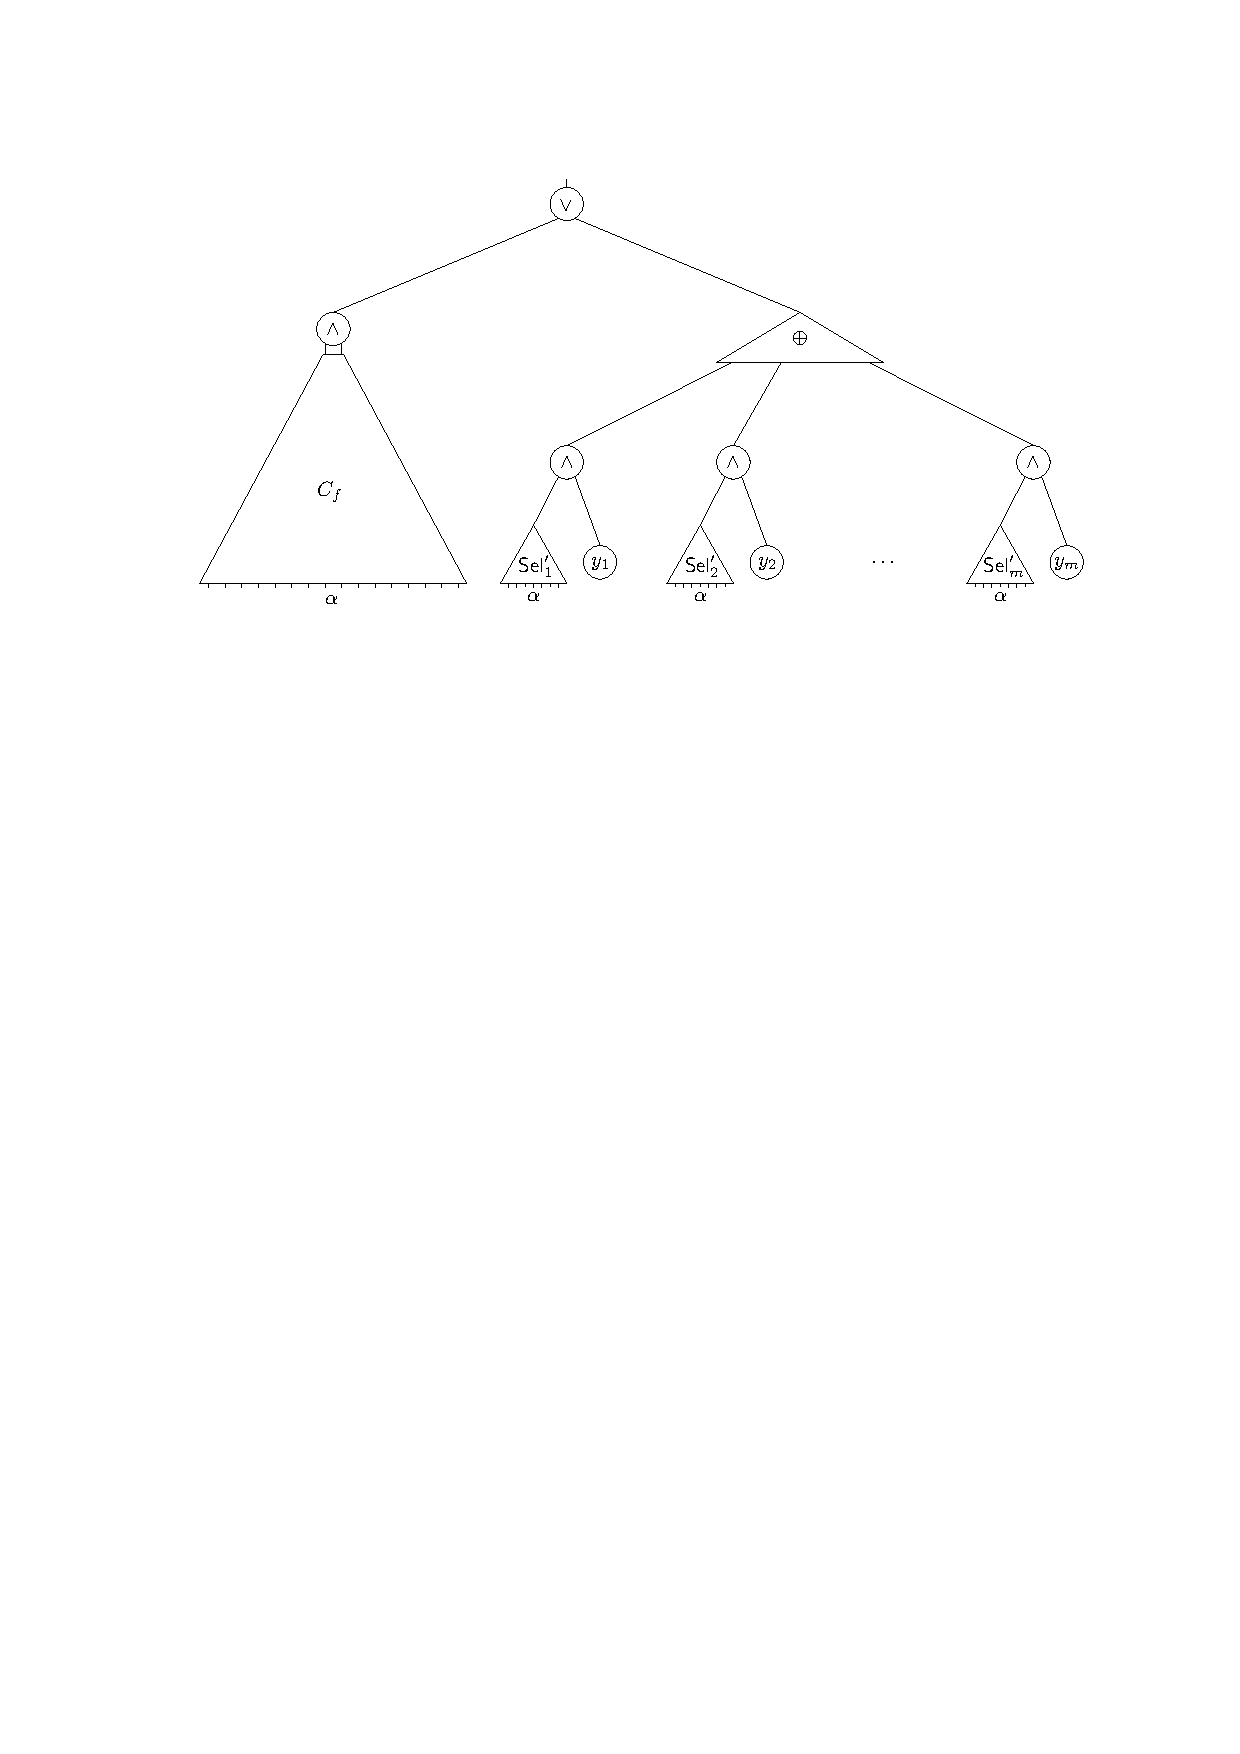
\includegraphics[width=\linewidth,height=\textheight,keepaspectratio]{fig/circuit-restricted.pdf}
    \caption{A schematic depiction of the formula after hitting it
      with the described restriction.}
    \label{fig:circuit-restricted}
  \end{figure}

  Note that this implements the intended semantics: for each
  input $\alpha \in \set{0,1}^n$ the selector circuits output $1$ on
  some variables $y_i$ which are then \emph{xor}'ed, and the
  restricted circuit outputs
  \begin{align}
    \bigoplus_{i \in N(\alpha)} y_i \eqcomma
  \end{align}
  unless $C_f(\alpha) \neq \bot$, in which case the output of the
  circuit is $f(\alpha)$ and all selector circuits output $0$. We
  require that $s$ is larger than the size of the described circuit
  which is of size $O\big(m \cdot \poly(n, k)\big) + s/2$.

  We have the intended semantics of the circuit and need to ensure the
  furthermore property: that the restricted formula is over few
  variables. First, since the selector circuits $\sel'_i$ are fixed,
  all evaluation variables for these subcircuits can be fixed to
  constants. The same holds for the circuit $C_f$. Similarly, since
  the $y_i$ gate always carries the value of the $y_i$ variable, all
  $2^n \cdot m$ wire variables corresponding to the $Y$ variables can
  be substituted by the corresponding $y_i$ variable and are thus
  restricted away.

  After these restrictions the only evaluation variables left are
  those for the evaluation of the $\oplus$ circuit.  For $\alpha$ such
  that $C_f(\alpha) \neq \bot$, the selector circuits are hard-wired
  to $0$ and in particular the inputs to the $\oplus$ circuit is
  hard-wired to $0$, meaning that these evalation variables can be
  restricted away.

  There remains then only the $O(t \cdot m)$ evaluation variables
  corresponding to the evaluation of the $\oplus$ circuit for inputs
  $\alpha$ such that $C_f(\alpha) = \bot$. Let us, without loss of
  generality, use an \emph{xor}-circuit which iteratively \emph{xor}s
  each variable.  Concretely, let it have subcircuits $\chi_i$ where
  $\chi_1 = \sel'_1 \wedge y_1$ and
  $\chi_{i} = \chi_{i-1} \oplus (\sel'_i \wedge y_i)$ for $i > 1$, and
  $\chi_m$ is the overall output of the $\oplus$ circuit.

  The only observation required is that if the circuit
  $\sel'_i(\alpha) = 0$, then $\chi_i$ gets a $0$ as input from index
  $i$, independent of the value of $y_i$. Hence the output wire
  variable of the circuit $\chi_i$ indexed by the input $\alpha$ can
  be substituted by the output of the circuit $\chi_{i-1}$. Hence for
  each $\alpha$ such that $C_f(\alpha) = \bot$, we can reduce the
  number of free wire variables indexed by $\alpha$ to $O(k)$, as each
  $\oplus$-constraint is over at most $k$ variables.  As $C_f$ outputs
  $\bot$ on at most $t$ inputs, we end up with a restriction leaving
  only a total of $O(t \cdot k + m)$ remaining variables in the
  restricted formula.

  This completes the description of the restriction $\rho$.  The only
  part that remains is to verify that $\rho$ is natural,
  $k$-determined, and $m$-independent.  That $\rho$ is natural is
  immediate -- it does not substitute any structural variable by an
  evaluation variable.  For $k$-determinedness, note that for a fixed
  input $\alpha$ at most $k$ selector circuits output $1$, and thus
  for every gate $u$ the value of $\outwire_\alpha(u)$ as a function
  of $Y$ can be computed by a function over those $k$ variables.
  Finally, each assignment to the remaining structure variables $Y$
  gives a valid circuit and thus $\rho$ is $m$-independent.
\end{proof}

We are ready to prove the degree lower bound, restated here for
convenience.

\MainDegree*

\begin{proof}
  Let $G = (U, V, E)$ be an explicit bipartite graph as in
  \cref{thm:expander}, with $U = \{0,1\}^n$,
  $k = O_{\gamma}\big((n \log r)^{1 + 1/\gamma}\big)$, and
  $|V| \le k^2 r^{1+\gamma}$ for parameters $\gamma > 0$ and
  $r \le 2^n$ to be fixed later. Apply \cref{lem:restriction} with $t=2^n$ along with
  $C_f = \bot$ to obtain, for $s \ge m \cdot \poly(n, k)$, a natural
  $m$-independent $k$-determined variable substitution $\rho$ for
  $\circuit_s(f)$ such that
  $\gout_{s, \alpha}(Y) = \oplus_{i \in N(\alpha)} y_i$. In words, the
  circuit of the restricted formula on input $\alpha$ computes an
  \emph{xor} of the neighborhood of the vertex $\alpha$ of $G$.

  Apply \cref{lem:circuit-to-poly} to $\rho$ to conclude that if there
  is an SoS refutation of $\restrict{\circuit_s(f)}{\rho}$ of degree
  $d$, then there is a degree $d \cdot k$ SoS refutation of the system
  of polynomial equations computing
  \begin{align}
    \nonumber
    \calP_G
    &= \Big\{
    \bigoplus_{i \in N(\alpha)} y_i = f(\alpha)
    :
    \alpha \in \set{0,1}^n
    \Big\}\,
    \cup
    \set{
    y_i^2 = y_i\mid i \in [m]
    }
    \eqperiod
  \end{align}
%
  As the graph $G$ is a strong expander, we can apply
  \cref{thm:sos-xor} to get an SoS degree lower bound of $\Omega(r)$
  for the XOR-CSP instance $\calP_G$ defined over $G$, which in turn
  gives us an $\Omega(r/k)$ degree lower bound for the
  $\restrict{\circuit_s(f)}{\rho}$ formula and hence also for the
  unrestricted formula.

  Let us fix the parameters. We want to choose $r$ as large as
  possible. However, the larger we choose $r$, the larger $m$ may
  become, since \cref{thm:expander} only guarantees that
  $m \le k^2 r^{1+\gamma}$. Let us analyze how large $r$ can be chosen
  in terms of $n$ and $s$.

  Note that $k = \poly_\gamma(n)$, where we use that $r \le 2^n$, and we write
  $\poly_\gamma(n)$ to denote some polynomial in $n$ whose degree and
  coefficients may depend on $\gamma$. Hence we may choose
  \begin{align}
    m = \frac{s}{\poly_{\gamma}(n)} \eqcomma
  \end{align}
  according to the requirement on $s$ in \cref{lem:restriction}.  From
  the guarantees of \cref{thm:expander} we know that
  $r \ge (m/k^2)^{1/(1+\gamma)}$. Substituting $m$ according to the
  previous equation we get that
  \begin{align}
    r
    \ge
    \left(
    \frac{s}{
    k^2 \poly_{\gamma}(n)
    }
    \right)^{\frac{1}{1 + \gamma}}
    =
    \frac{s^{1/(1 + \gamma)}}{\poly_{\gamma}(n)} \eqperiod
  \end{align}
  Hence if we choose $\gamma$ small enough so that
  $\frac{1}{1+\gamma} > 1-\eps/2$ and then require $s$ to be large
  enough such that the final $\poly_{\gamma}(n)$ is at most
  $s^{\eps/2}$, we obtain the claimed lower bound.
\end{proof}

In the following we prove the claimed size lower bound.

\MainSize*

\begin{proof}
  Apply \cref{lem:restriction} with the graphs from
  \cref{thm:expander} as in the proof of \cref{thm:main-degree}. We
  get a natural $m$-independent $k$-determined variable substitution
  $\rho$ and the formula $\restrict{\circuit_s(f)}{\rho}$ over
  $O(t \cdot k + m)$ variables.  To this formula we then apply
  \cref{lem:circuit-to-poly} to obtain a degree lower bound of
  $\Omega(r/k)$, akin to the proof of \cref{thm:main-degree}. By
  setting the parameters as in the aforementioned proof we get the
  same degree lower bound of $\Omega_\eps(s^{1-\eps/3})$ for the
  formula $\restrict{\circuit_s(f)}{\rho}$. As this formula is over
  few variables we can apply \cref{thm:tradeoff} to obtain an SoS size
  lower bound of
  $\exp \Big( \Omega_\eps\big((s^{1- \eps/3} - 3k)^2/(t \cdot k +
  m)\big) \Big)$ for the restricted formula. As variable substitutions
  may only decrease the size of a refutation, the same lower bound
  also holds for the unrestricted formula. We obtain the desired lower
  bound by choosing $s$ large enough such that
  $s^{\eps/3} \ge k = \poly_\eps(n)$ and by recalling that
  $t \ge s \ge m$. 
\end{proof}

\newcommand{\etalchar}[1]{$^{#1}$}
\begin{thebibliography}{KMOW17}

\bibitem[ABRW04]{ABRW04Pseudorandom}
Michael Alekhnovich, Eli {Ben-Sasson}, Alexander~A. Razborov, and Avi
  Wigderson.
\newblock Pseudorandom generators in propositional proof complexity.
\newblock {\em SIAM Journal on Computing}, 34(1):67\nobreakdash--88, 2004.
\newblock Preliminary version in \emph{FOCS~'00}.

\bibitem[AH19]{AH18SosTradeoff}
Albert Atserias and Tuomas Hakoniemi.
\newblock {Size-Degree Trade-Offs for Sums-of-Squares and Positivstellensatz
  Proofs}.
\newblock In Amir Shpilka, editor, {\em 34th Computational Complexity
  Conference (CCC 2019)}, volume 137 of {\em Leibniz International Proceedings
  in Informatics (LIPIcs)}, pages 24:1--24:20, Dagstuhl, Germany, 2019. Schloss
  Dagstuhl--Leibniz-Zentrum fuer Informatik.

\bibitem[AOW15]{AOW15}
S.~R. Allen, R.~ODonnell, and D.~Witmer.
\newblock How to refute a random csp.
\newblock In {\em 2015 IEEE 56th Annual Symposium on Foundations of Computer
  Science (FOCS)}, pages 689--708, Los Alamitos, CA, USA, oct 2015. IEEE
  Computer Society.

\bibitem[Ber82]{B82}
S.~J. Berkowitz.
\newblock On some relationships between monotone and non-monotone circuit
  complexity.
\newblock Technical report, Technical Report, University of Toronto, 1982.

\bibitem[BHK{\etalchar{+}}16]{BHKKMP16clique}
B.~{Barak}, S.~B. {Hopkins}, J.~{Kelner}, P.~{Kothari}, A.~{Moitra}, and
  A.~{Potechin}.
\newblock A nearly tight sum-of-squares lower bound for the planted clique
  problem.
\newblock In {\em 2016 IEEE 57th Annual Symposium on Foundations of Computer
  Science (FOCS)}, pages 428--437, 2016.

\bibitem[BT06]{BT06}
Andrej Bogdanov and Luca Trevisan.
\newblock Average-case complexity.
\newblock {\em Foundations and Trends in Theoretical Computer Science},
  2(1):1--106, 2006.

\bibitem[BW06]{BW06}
Amos Beimel and Enav Weinreb.
\newblock Monotone circuits for monotone weighted threshold functions.
\newblock {\em Inf. Process. Lett.}, 97(1):12–18, jan 2006.

\bibitem[GHP02]{GHA02proofs}
Dima Grigoriev, Edward~A. Hirsch, and Dmitrii~V. Pasechnik.
\newblock Complexity of semi-algebraic proofs.
\newblock In {\em STACS 2002}, pages 419--430, Berlin, Heidelberg, 2002.
  Springer Berlin Heidelberg.

\bibitem[Gol20]{Goldreich2020}
Oded Goldreich.
\newblock {\em On (Valiant's) Polynomial-Size Monotone Formula for Majority},
  pages 17--23.
\newblock Springer International Publishing, Cham, 2020.

\bibitem[Gri01]{gri01xor}
Dima Grigoriev.
\newblock Linear lower bound on degrees of positivstellensatz calculus proofs
  for the parity.
\newblock {\em Theoretical Computer Science}, 259(1):613 -- 622, 2001.

\bibitem[GUV09]{GUV09Unbalanced}
Venkatesan Guruswami, Christopher Umans, and Salil Vadhan.
\newblock Unbalanced expanders and randomness extractors from
  {P}arvaresh--{V}ardy codes.
\newblock {\em Journal of the ACM}, 56(4):20:1\nobreakdash--20:34, July 2009.
\newblock Preliminary version in \emph{CCC~'07}.

\bibitem[GW95]{GW95}
Michel~X. Goemans and David~P. Williamson.
\newblock Improved approximation algorithms for maximum cut and satisfiability
  problems using semidefinite programming.
\newblock {\em J. {ACM}}, 42(6):1115--1145, 1995.

\bibitem[Hir18]{Hi18}
Shuichi Hirahara.
\newblock Non-black-box worst-case to average-case reductions within np.
\newblock In {\em 2018 IEEE 59th Annual Symposium on Foundations of Computer
  Science (FOCS)}, pages 247--258, 2018.

\bibitem[KC00]{KC00}
Valentine Kabanets and Jin-Yi Cai.
\newblock Circuit minimization problem.
\newblock In {\em Proceedings of the Thirty-Second Annual ACM Symposium on
  Theory of Computing}, STOC '00, page 73–79, New York, NY, USA, 2000.
  Association for Computing Machinery.

\bibitem[KMOW17]{kmow17anycsp}
Pravesh~K. Kothari, Ryuhei Mori, Ryan O’Donnell, and David Witmer.
\newblock Sum of squares lower bounds for refuting any csp.
\newblock In {\em Proceedings of the 49th Annual ACM SIGACT Symposium on Theory
  of Computing}, STOC 2017, page 132–145, New York, NY, USA, 2017.
  Association for Computing Machinery.

\bibitem[KMS98]{KMS98}
David Karger, Rajeev Motwani, and Madhu Sudan.
\newblock Approximate graph coloring by semidefinite programming.
\newblock {\em J. ACM}, 45(2):246–265, mar 1998.

\bibitem[Kra01]{Krajicek01}
Jan Krajíček.
\newblock On the weak pigeonhole principle.
\newblock {\em Fundamenta Mathematicae}, 170(1-2):123--140, 2001.

\bibitem[MPW15]{MPW15SumOfSquaresPlantedClique}
Raghu Meka, Aaron Potechin, and Avi Wigderson.
\newblock Sum-of-squares lower bounds for planted clique.
\newblock In {\em Proceedings of the 47th Annual ACM Symposium on Theory of
  Computing ({STOC}~'15)}, pages 87\nobreakdash--96, June 2015.

\bibitem[MW15]{MW15}
Cody~D. Murrayand and R.~Ryan Williams.
\newblock {On the (Non) NP-Hardness of Computing Circuit Complexity}.
\newblock In David Zuckerman, editor, {\em 30th Conference on Computational
  Complexity (CCC 2015)}, volume~33 of {\em Leibniz International Proceedings
  in Informatics (LIPIcs)}, pages 365--380, Dagstuhl, Germany, 2015. Schloss
  Dagstuhl--Leibniz-Zentrum fuer Informatik.

\bibitem[Pot20]{potechin20}
Aaron Potechin.
\newblock {Sum of Squares Bounds for the Ordering Principle}.
\newblock In Shubhangi Saraf, editor, {\em 35th Computational Complexity
  Conference (CCC 2020)}, volume 169 of {\em Leibniz International Proceedings
  in Informatics (LIPIcs)}, pages 38:1--38:37, Dagstuhl, Germany, 2020. Schloss
  Dagstuhl--Leibniz-Zentrum f{\"u}r Informatik.

\bibitem[PR04]{PitRaz04}
Toniann Pitassi and Ran Raz.
\newblock Regular resolution lower bounds for the weak pigeonhole principle.
\newblock {\em Combinatorica}, 24(3):503--524, 2004.
\newblock Preliminary version in \emph{STOC~'01}.

\bibitem[Raz98]{Razborov98}
Alexander~A. Razborov.
\newblock Lower bounds for the polynomial calculus.
\newblock {\em Computational Complexity}, 7(4):291\nobreakdash--324, December
  1998.

\bibitem[Raz04a]{Raz04}
Ran Raz.
\newblock Resolution lower bounds for the weak pigeonhole principle.
\newblock {\em J. {ACM}}, 51(2):115--138, 2004.

\bibitem[Raz04b]{Razborov04ResolutionLowerBoundsPM}
Alexander~A. Razborov.
\newblock Resolution lower bounds for perfect matching principles.
\newblock {\em Journal of Computer and System Sciences},
  69(1):3\nobreakdash--27, August 2004.
\newblock Preliminary version in \emph{CCC~'02}.

\bibitem[Raz15]{Razborov15PRG}
Alexander~A. Razborov.
\newblock Pseudorandom generators hard for \mbox{$k$-{DNF}} resolution and
  polynomial calculus resolution.
\newblock {\em Annals of Mathematics}, 181(2):415\nobreakdash--472, March 2015.

\bibitem[Raz21]{razborov21youtube}
Alexander Razborov.
\newblock {P}, {NP} and {Proof Complexity}.
\newblock \url{https://youtu.be/ZVL_HsPC4xE?t=2646}, 2021.
\newblock Accessed April 2022.

\bibitem[Raz22]{razborov22website}
Alexander Razborov.
\newblock Open problems.
\newblock \url{https://people.cs.uchicago.edu/~razborov/teaching/index.html},
  2022.
\newblock Accessed April 2022.

\bibitem[RRS17]{RRS17}
Prasad Raghavendra, Satish Rao, and Tselil Schramm.
\newblock Strongly refuting random csps below the spectral threshold.
\newblock In {\em Proceedings of the 49th Annual ACM SIGACT Symposium on Theory
  of Computing}, STOC 2017, page 121–131, New York, NY, USA, 2017.
  Association for Computing Machinery.

\bibitem[RWY02]{RazbWigYao02}
Alexander~A. Razborov, Avi Wigderson, and Andrew~Chi{-}Chih Yao.
\newblock Read-once branching programs, rectangular proofs of the pigeonhole
  principle and the transversal calculus.
\newblock {\em Combinatorica}, 22(4):555--574, 2002.
\newblock Preliminary version in \emph{STOC~'97}.

\bibitem[Val84]{Valiant84}
Leslie~G. Valiant.
\newblock Short monotone formulae for the majority function.
\newblock {\em J. Algorithms}, 5:363--366, 1984.

\end{thebibliography}
\end{document}
